\documentclass[text07.tex]{subfiles}
\begin{document}
% \refstepcounter{Exercise}
% \clearpage\subsection*{2−3　\theExercise　友だちのホームページを見てみよう}

%
% subsection 6.3.3
%
\subsection{友だちのホームページを見てみよう}\label{friend}
% \addtocounter{Exercise}{-1}\refstepcounter{Exercise}\label{friend}
% \clearpage\subsection*{2−3友だちのホームページを見てみよう}

\begin{center}
        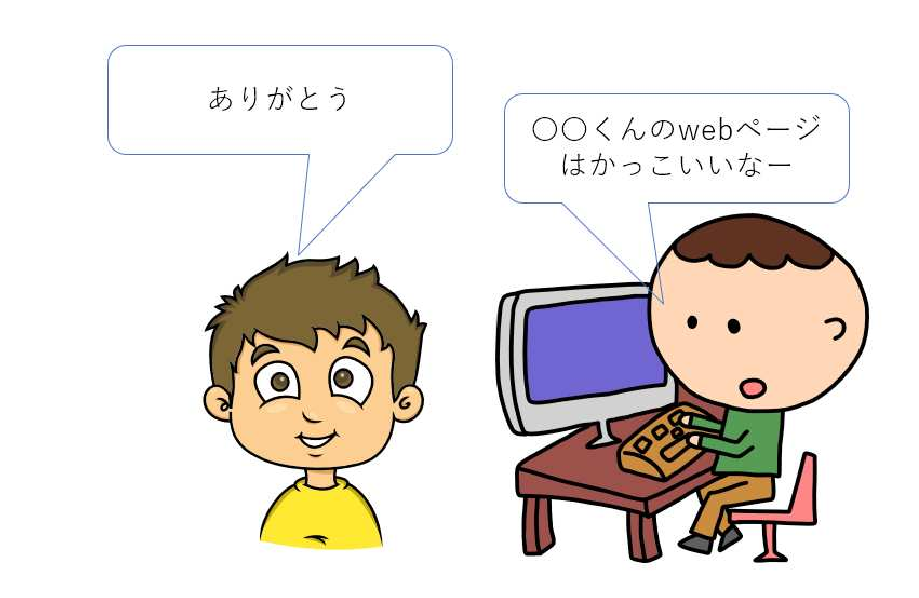
\includegraphics[width=10.423cm]{../../asset/image/ome7-img042}
\end{center}

\bigskip

\begin{enumerate}
    \item \ruby{左隣}{ひだりどなり}の友達のIPアドレスを確認しよう。

	友達のターミナルで次のコマンドをうってもらいましょう。

	hostname -I

	そのIPアドレスをメモしましょう。

	[\underline{　　　　}さんのIP:\underline{　　　　　　　　　　　　　　}]


	\bigskip

	\item 友達のウェブページを見て見ましょう。

	自分のサーバを見るときは

	\url{http://localhost:3000/}

	でした。localhostというのが自分のサーバという意味でした。

	今回は友達のサーバを見たいのでlocalhostの代わりに友達のIPアドレスを打ちましょう。

	\url{http://xxx.xxx.xxx.xxx:3000/}

	\url{http://xxx.xxx.xxx.xxx:3000/index.html}

	をブラウザのアドレスバーに打ってみましょう。

	もし左隣の友達のIPアドレスが192.162.33.5だったら

	\url{http://192.162.33.5:3000/index.html}

	となります。

	友達のウェブページが表示されたら成功です！

	\begin{center}
        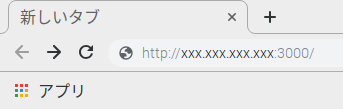
\includegraphics[width=10.659cm]{../../asset/image/ome7-img043.png}
	\end{center}

\end{enumerate}

% 1.
% \ruby{左隣}{ひだりどなり}の友達のIPアドレスを確認しよう。

% \ \ 友達のターミナルで次のコマンドをうってもらいましょう。

% \ \ hostname -I

% \ \ そのIPアドレスをメモしましょう。

% \ \ [\underline{　　　　}さんのIP:\underline{　　　　　　　　　　　　　　}]


% \bigskip

% 2.友達のウェブページを見て見ましょう。

% \ \ 自分のサーバーを見るときは

% \ \ 　\url{http://localhost:3000/}

% \ \ でした。localhostというのが自分のサーバーという意味でした。

% \ \ 今回は友達のサーバーを見たいのでlocalhostの代わりに友達のIPアドレスを打ちましょう。

% \ \ 　\url{http://xxx.xxx.xxx.xxx:3000/}

% \ \ \ 　\url{http://xxx.xxx.xxx.xxx:3000/index.html}

% \ \ をブラウザのアドレスバーに打ってみましょう。

% \ \ もし左隣の友達のIPアドレスが192.162.33.5だったら

% \ \ 　\url{http://192.162.33.5:3000/index.html}

% \ \ となります。

% \ \ 友達のウェブページが表示されたら成功です！


% \bigskip


% \centering
% 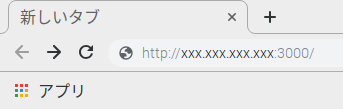
\includegraphics[width=10.659cm]{../../asset/image/ome7-img043.png}
% \flushleft

\clearpage
% \subsection
{\bfseries 	注意}

\ref{friend}の友達のホームページを見てみようでは、以下の図のように同じルータにつながっているラズベリーパイが公開しているホームページは、見ることができます。
\ruby{基本}{きほん}同じグループの子たちのホームページは見れるので確認してみてください。

\begin{center}
	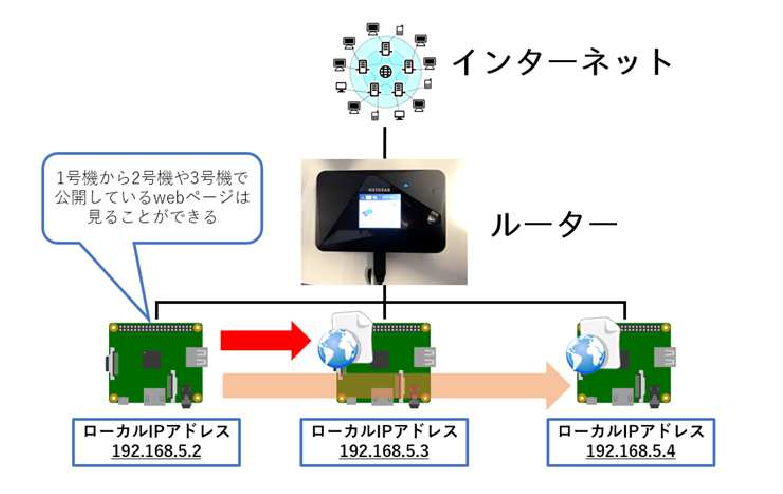
\includegraphics[width=0.75\textwidth]{../../asset/image/ome7-img044}
\end{center}

\bigskip

また、他のルータに接続しているラズベリーパイが公開しているホームページは今回みることができません。実際に試してみても面白いと思います。


\bigskip

\begin{center}
	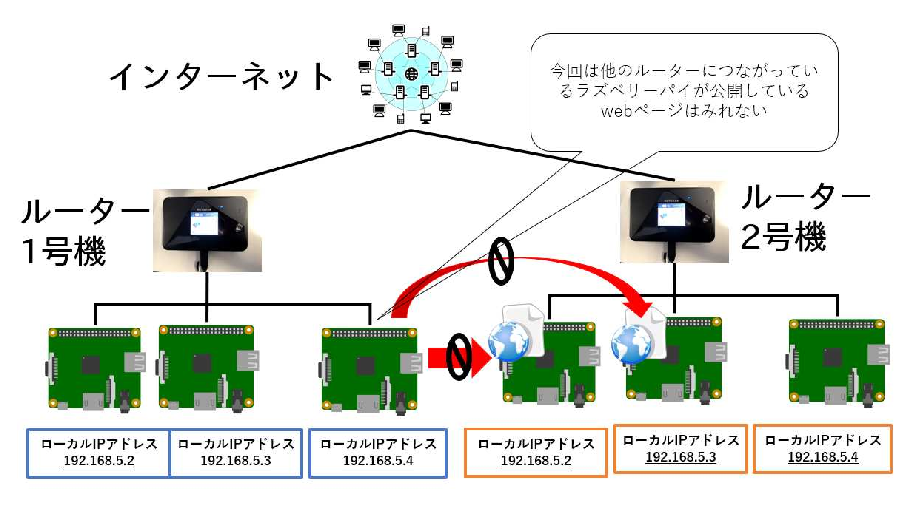
\includegraphics[width=0.75\textwidth]{../../asset/image/ome7-img045}
\end{center}

\bigskip

\begin{tcolorbox}[title=\useOmetoi,breakable]\label{Q:otherHP}
  \begin{enumerate}
    \addquiz{他のグループの友達のホームページを見て、自分とは違うWi-Fiルータに接続している友達のホームページは見れたかどうか答えに書こう。}
  \end{enumerate}
\end{tcolorbox}

\clearpage

% \if0


% 	参考　接続できるネットワーク(Wi-Fiルータ)

% 	NTGR-4643\ \ \ \ パスワード　33995460

% 	NTGR-3EBC\ \ \ \ パスワード　34986626

% 	NTGR-3DFC\ \ \ \ パスワード　36976828

% \fi
\end{document}
